\documentclass[lang=en,11pt]{elegantbook}
\usepackage{amsmath}
\renewcommand{\theequation}{\arabic{equation}}
%\renewcommand\thechapter{\Roman{chapter}}
%\renewcommand\thesection{\arabic{section}}
%\renewcommand\thesection{\arabic{subsection}}
\title{Principles of optics}
\subtitle{SEVEBTH(EXPANDED)EDITION}

\author{Max Born \& Emil Wolf}
\institute{CAMBRIDGE UNIVERSITY PRESS}
\date{}
\version{3.10}
\bioinfo{Bio}{HUIKERR}

\extrainfo{Victory won\rq t come to us unless we go to it. }

\logo{logo.png}
\cover{cover.jpg}

\begin{document}
	
	\maketitle
	
	\frontmatter
	\tableofcontents
	
	\mainmatter
	\chapter{Basic properties of the electromagnetic field}
	\section{The electromagnetic field}
	\subsection{Maxwell's equations}
	THE state of excitation which is established in space by the presence of electric charges is said to constitute \textit{an electromagnetic field}. It is represented by two vectors,\textbf{E} and \textbf{B},called the \textit{electric vector} and the \textit{magnetic induction} respectively.\footnote{In elementary considerations \textbf{E} and \textbf{H} are, for historical reasons, usually regarded as the basic field vectors, and \textbf{D} and \textbf{B} as describing the influence of matter. In general theory, however, the present interpretation is compulsory for reasons connected with the electrodynamics of moving media.\par The four Maxwell equations \eqref{1-1}-\eqref{1-4} can be divided into two sets of equations, one consisting of two homogeneous equations (right-hand side zero), containing \textbf{E} and \textbf{B}, the other of two non-homogeneous equations (right-hand side different from zero), containing \textbf{D} and \textbf{H}. If a coordinate transformation of space and time (relativistic Lorentz transformation) is carried out, the equations of each group transform together, the equation remaining unaltered in form if \textbf{j}/c and $\rho$ are transformed as a four-vector, and each of the pairs \textbf{E, B} and \textbf{D, H} as a six-vector (anti-symmetric tensor of the second order). Since the non-homogeneous set contains charges and currents (which represent the influence of matter), one has to attribute the corresponding pair (\textbf{D, H}) to the influence of matter. It is, however, customary to refer to \textbf{H} and not to be \textbf{B} as the \textit{magnetic field vector}, we shall conform to this terminology when there is no risk of confusion. }\par
	To describe the effect of the field on material objects, it is necessary to introduce a second set of vectors, viz. \textit{the electric current density} \textbf{j}, \textit{the electric displacement} \textbf{D}, and \textit{the magnetic vector} \textbf{H}.\par 
	The space and time derivatives of the five vectors are related by \textit{Maxwell's equations}, which hold at every point in whose neighbourhood the physical properties of the medium are continuous:\footnote{The so-called Gaussian system of units is used here, i.e. the electrical quantities (\textbf{E, D, j} and $\rho$) are measured in electrostatic units, and the magnetic quantities (\textbf{H} and \textbf{B}) in electromagnetic units. The constant c in \eqref{1-1} and \eqref{1-2} related the units of charge in the two systems; it is the velocity of light in the vacuum and is approximately equal to $3\times10^{10}cm/s$.(A more accurate value is given in \S1.2.)}
	\begin{equation}
	curl\ \textbf{H}-\frac{1}{c}\dot{\textbf{D}}=\frac{4\pi}{c}\textbf{j},
	\label{1-1}
	\end{equation}
	\begin{equation}
	curl\ \textbf{E}+\frac{1}{c}\dot{\textbf{B}}=0,
	\label{1-2}
	\end{equation}
	the dot denoting differentiation with respect to time.\par
	They are supplemented by two scalar relation:
	\begin{equation}
	div\ \textbf{D}=4\pi\rho,
	\label{1-3}
	\end{equation}
	\begin{equation}
	div\ \textbf{B}=0.
	\label{1-4}
	\end{equation}
	Eq.\eqref{1-3}may be regarded as a defining equation for the electric charge density $\rho$ and \eqref{1-4} may be said to imply that no free magnetic poles exist.\par 
	From \eqref{1-1} it follows (since $div\ curl\equiv 0$)
	\begin{equation*}
	div\ \textbf{j}=-\frac{1}{4\pi}div\ \dot{\textbf{D}},
	\end{equation*}
	or, using \eqref{1-3},
	\begin{equation}
	\frac{\partial\rho}{\partial t}+div\ \textbf{j}=0.
	\label{1-5}
	\end{equation}
	By analogy with a similar relation encountered in hydrodynamics, \eqref{1-5} is called the \textit{equation of continuity}. It expresses the fact that the charge is conserved in the neighbourhood of any point. For if one integrates \eqref{1-5} over any region of space, one obtains, with the help of Gauss' theorem,
	\begin{equation}
	\frac{\mathrm{d}}{\mathrm{d} t} \int \rho \mathrm{d} V+\int \mathbf{j} \cdot \mathbf{n} \mathrm{d} S=0
	\label{1-6}
	\end{equation}
	the second integral being taken over the surface bounding the region and the first throughout the volume, \textbf{n} denoting the unit outward normal. The equation implies that the total charge
	\begin{equation}
	e=\int \rho dV
	\label{1-7}
	\end{equation}
	contained within the domain can only increase on account of the flow of electric current
	\begin{equation}
	\jmath=\int \mathbf{j}\cdot\mathbf{n}dS
	\label{1-8}
	\end{equation}
	\par 
	If all the field quantities are independent of time, and if, moreover, there are no currents($\textbf{j}=0$), the field is said to be \textit{static}. If all the field quantities are time independent, but currents are present ($\mathbf{j}\neq 0$), one speaks of a \textit{stationary field}. In optical field the field vectors are very rapidly varying functions of time, but the sources of the field are usually such that, when average over any macroscopic time interval are considered rather than the instantaneous values, the properties of the field are found to be independent of the instant of time at which the average is taken. The word \textit{stationary} is often used in a wider sense to describe a field of this type. An example is a field constituted by the steady flux of radiation(say from a distant star)through an optical system. 
	
	\subsection{Material equations}
	The Maxwell equations (\ref{1-1}-\ref{1-4}) connect the five basic quantities \textbf{E, H, B, D} and \textbf{j}. To allow a unique determination of the field vectors from a given distribution of currents and charges, these equations must be supplemented by relations which describe the behaviour of substances under the influence of the field. These relations are known as \textit{material equations}\footnote{There is an alternative way of describing the behaviour of matter. Instead of the quantities $\varepsilon=D/E,\mu=B/H$ one considers the differences \textbf{D-E} and \textbf{B-H}; these have a simpler physical significance and will be discussed in Chapter II.} (or \textit{constitutive relation}). In general they are rather complicated; but if the field is time-harmonic (see \S1.4.3), and if the bodies are at rest, or in very slow motion relation to each other, and if the material is \textit{isotropic} (i.e. when its physical properties at each point are independent of direction), they take usually the relatively simple form\footnote{The more general relations, applicable also to moving bodies, are studied in the theory of relativity. We shall only need the following result from the more general theory: that in the case of moving charges there is, in addition to the conduction current $\sigma\textbf{E}$,a convection current $\rho\textbf{v}$,where \textbf{v} is the velocity of the moving charges and $\rho$ the charge density (cf.p.9).}
	\begin{equation}
	\mathbf{j}=\sigma\mathbf{E},
	\label{1-9}
	\end{equation}
	\begin{equation}
	\mathbf{D}=\varepsilon\mathbf{E},
	\label{1-10}
	\end{equation}
	\begin{equation}
	\mathbf{B}=\mu\mathbf{H}.
	\label{1-11}
	\end{equation}
	Here $\sigma$ is called the \textit{specific conductivity}, $\varepsilon$ is known as the \textit{dielectric constant}(or permittivity) and $\mu$ is called the \textit{magnetic permeability}.\par
	Eq.\eqref{1-9} is the differential form of Ohm's law. Substances for which $\sigma\neq0$(or more precisely is not negligibly small;the precise meaning of this cannot, however, be discussed here) are called \textit{conductors}. Metals are very good conductors, but there are other classes of good conducting materials such as ionic solutions in liquids and also in solids. In metals the conductivity decreases with increasing temperature. However, in other classes of materials, known as  \textit{semiconductors} (e.g. germanium), conductivity increases with temperature over a wide range.\par
	Substances for which $\sigma$ is negligibly small are called \textit{insulators} or \textit{dielectrics}. Their electric and magnetic properties are then completely determined by $\varepsilon$ and $\mu$. For most substances the magnetic permeability $\mu$ is practically unity. If this is not the case, i.e. if $\mu$ differs appreciable form unity, we say that the substance is \textit{magnetic}. In particular, if $\mu>1$, the substance is said to be \textit{para-magnetic} (e.g. platinum, Oxygen, nitrogen dioxide), while if $\mu<1$ it is said to be \textit{diamagnetic} (e.g. bismuth, copper, hydrogen, water).\par
	If the fields are exceptionally strong, such as are obtained, for example, by focusing light that is generated by a laser, the right-hand sides of the material equations may have to be supplemented by terms involving components of the field vectors in powers higher than the first.\footnote{Nonlinear relationship between the displacement vector \textbf{D} and the electric field \textbf{E} was first demonstrated in this way by P.A.Franken, A.E.Hill, C.W.Peters and G.Weinrich, \textit{Phys.Rev.Lett}, 7(1961), 118.\par
		For systematic treatments of nonlinear effects see N.Bloembergen, \textit{Nonlinear Optics} (Cambridge, Cambridge University Press, 1990) or R.W.Boyd, \textit{Nonlinear Optics} (Boston, Academic Press, 1992).}
	In many cases the quantities $\sigma$, $\varepsilon$ and $\mu$ will be independent of field strengths; in other cases, however, the behaviour of the material cannot be described in such a simple way. Thus, for example, in a gas of free ions the current, which is determined by the mean speed of the ions, depends, at any moment, not on the instantaneous value of \textbf{E}, but on all its previous values. Again, in so-called \textit{ferromagnetic} substances (substances which are very highly magnetic, e.g. iron, cobalt and nickel) the value of the magnetic induction \textbf{B} is determined by the past history of the field \textbf{H} rather than by its instantaneous value. The substance is then said to exhibit \textit{hysteresis}. A similar history-dependence will be found for the electric displacement in certain dielectric materials. Fortunately hysteretic effects are rarely significant for the high-frequency field encouraged in optics.\par
	In the main part of this book we shall study the propagation in substances which light can penetrate without appreciable weakening (e.g. air, glass). Such substances are said to be \textit{transparent} and must be electrical nonconductors ($\sigma=0$), since conduction implies the evolution of Joule heat (see \S1.1.4) and therefore loss of electromagnetic energy. Optical properties of conducting media will be discussed in Chapter 14.
	
	\subsection{Boundary conditions at a surface of discontinuity}
	Maxwell's equations were only stated for regions of space throughout which the physical properties of the medium (characterized by $\varepsilon$ and $\mu$) are continuous. In optics one often deals with situations in which the properties change abruptly across one or more surfaces. The vectors \textbf{E, H, B} and \textbf{D} may then be expected also to become discontinuous, while $\rho$ and \textbf{j} will degenerate into corresponding surface quantities. We shall derive relations describing the transition across such a discontinuity surface.\par
	Let us replace the sharp discontinuity surface \textit{T} by a thin transition layer within which $\varepsilon$ and $\mu$ vary rapidly but continuously from their values near \textit{T} on one side to their value near \textit{T} on the other. Within this layer we construct a small near-cylinder, bounded by a stockade of normals to \textit{T}; roofed and floored by small areas $\delta A_!$ and $\delta A_2$ on each side of \textit{T}, at constant distance from it, measured along their common normal \eqref{fig:1-1}. Since \textbf{B} and its derivatives may be assumed to be continuous throughout this cylinder, we may apply Gauss' theorem to the integral of div\ \textbf{B} taken throughout the volume of the cylinder and obtain, from \eqref{1-4},
	\begin{equation}
	\int div\ \mathbf{B}dV=\int\mathbf{B\cdot n}dS=0;
	\label{1-12}
	\end{equation}
	the second integral is taken over the surface of the cylinder, and \textbf{n} is the unit outward normal.\par
	Since the areas $\delta A_1$ and $\delta A_2$ are assumed to be small, \textbf{B} may be considered to have constants values $\mathbf{B^{(1)}}$ and $\mathbf{B^{(2)}}$) on $\delta A_1$ and $\delta A_2$, and \eqref{1-12} may then be replaced by
	\begin{figure}[htp!]
		\centering
		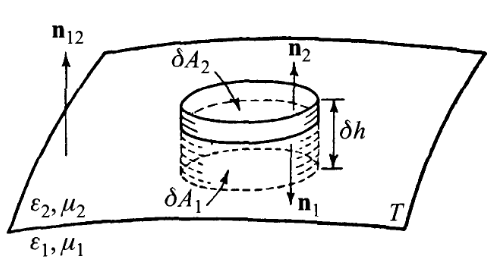
\includegraphics[scale=0.5]{image/fig1-1.png}
		\caption{Derivation of boundary conditions for the normal components of \textbf{B} and \textbf{D}.}
		\label{fig:1-1}
	\end{figure}
	\begin{equation}
	\mathbf{B^{(1)}\cdot n_{1}}\delta A_{1}+\mathbf{B^{(2)}\cdot n_{2}}\delta A_{2}+\text{contribution from walls}=0.
	\label{1-13}
	\end{equation}
	If the height $\delta h$ of the cylinder decreases towards zero, the transition layer shrinks into the surface and the contribution from the walls of the cylinder tends to zero, provided that there is no surface flux of magnetic induction. Such flux never occurs, and consequently in the limit,
	\begin{equation}
	(\mathbf{B^{(1)}\cdot n_{1}}+\mathbf{B^{(2)}\cdot n_{2}})\delta A=0,
	\label{1-14}
	\end{equation}
	$\delta A$ being the area in which the cylinder intersects \textit{T}. If $n_{12}$ is the unit normal pointing from the first into the second medium, then $\mathbf{n_{1}} = —\mathbf{n_{12}}, \mathbf{n_2} = \mathbf{n_{12}}$ and \eqref{1-14} gives
	\begin{equation}
	\mathbf{n_{12}}\cdot(\mathbf{B^{(2)}-\mathbf{B^{(1)}}})=0,
	\label{1-15}
	\end{equation}
	i.e. \textit{the normal component of the magnetic induction is continuous across the surface of discontinuity}.\par 
	The electric displacement \textbf{D} may be treated in a similar way, but there will be an additional term if charges are present. In place of \eqref{1-12} we now have from \eqref{1-3}
	\begin{equation}
	\int div\ \mathbf{D}dV=\int\mathbf{D\cdot n}dS=4\pi\int\rho dV.
	\label{1-16}
	\end{equation}
	As the areas $\delta A_1$ and $\delta A_2$ shrink together, the total charge remains finite, so that the volume density becomes infinite. Instead of the volume charge density $\rho$ the concept of surface charge density $\hat{\rho}$ must then be used. It is defined by\footnote{For later purposes we note a representation of the surface charge density and the surface current density in terms of the Dirac delta function (see Appendix IV). If the equation of the surface of discontinuity is $F(x, y, z)=0$, then
		%\begin{subequations}
			\begin{align}
			\rho &= \hat{\rho}|grad\ F|\delta(F),\tag{\ref{1-17}{a}} \label{1-17-a}\\
			\mathbf{j} &= \mathbf{\hat{j}}|grad\ F|\delta(F).\tag{\ref{1-18}{a}} \label{1-18-a}
			\end{align}
		%\end{subequations}	
 		These relations can immediately be verified by substituting from \eqref{1-17-a} and \eqref{1-18-a} into \eqref{1-17} and \eqref{1-18} and using the relation $dF=|grad\ F|dh$ and the sifting property of the delta function.}
	\begin{equation}
	\lim_{\substack{\delta h\rightarrow 0}}\int\rho dV=\int\hat{\rho}dA
	\label{1-17}
	\end{equation}
	We shall also need later the concept of surface current density $\mathbf{\hat{j}}$, defined in a similar way:
	\begin{equation}
	\lim_{\substack{\delta h\rightarrow 0}}\int\mathbf{j}dV=\int\mathbf{\hat{j}}dA
	\label{1-18}
	\end{equation}
	If the area $\delta A$ and the height $\delta h$ are taken sufficiently small, \eqref{1-16} gives
	\begin{equation*}
	\mathbf{D^{(1)}\cdot n_{1}}\delta A_{1}+\mathbf{D^{(2)}\cdot n_{2}}\delta A_{2}+\text{contribution from walls}=4\pi\hat{\rho}\delta A.
	\end{equation*}
	The contribution from the walls tends to zero with dh, and we therefore obtain in the
	limit as $dh\rightarrow0$,
	\begin{equation}
	\mathbf{n_{12}}(\mathbf{D^{(2)}}-\mathbf{D^{(1)}})=4\pi\hat{\rho}
	\label{1-19}
	\end{equation}
	\textit{i.e. in the presence of a layer of surface charge density $\hat{\rho}$ on the surface, the normal component of the electric displacement changes abruptly across the surface, by an amount equal to $4\pi\hat{\rho}$.}
	Next, we examine the behaviour of the tangential components. Let us replace the sharp discontinuity surface by a continuous transition layer. We also replace the cylinder of \eqref{fig:1-1} by a 'rectangular' area with sides parallel and perpendicular to \textit{T} \eqref{fig:1-2}.\par
	Let b be the unit vector perpendicular to the plane of the rectangle. Then it follows from \eqref{1-2} and from Stokes' theorem that
	\begin{equation}
	\int curl\ \mathbf{E\cdot b}dS=\int\mathbf{E}d\mathbf{r}=-\frac{1}{c}\int\mathbf{\dot{B}\cdot b}dS
	\label{1-20}
	\end{equation}
	the first and third integrals being taken throughout the area of the rectangle, and the	second along its boundary. If the lengths $P_1Q_1(=\delta{s1})$, and $P_2Q_2(=\delta{s2})$ are small, \textbf{E} may be replaced by constant values $\mathbf{E^{(1)}}$ and $\mathbf{E^{(2)}}$ along each of these segments. Similarly $\mathbf{\dot{B}}$ may be replaced by a constant value. Eq. \eqref{1-20} then gives
	\begin{equation}
	\mathbf{E^{(1)}\cdot t_1\delta{s1}}+\mathbf{E^{(2)}\cdot t_2\delta{s2}}+\text{contribution from ends}=-\frac{1}{c}\mathbf{\dot{B}\cdot b}\delta s\delta h,
	\label{1-21}
	\end{equation}
	where $\delta s$ is the line element in which the rectangle intersects the surface. If now the	height of the rectangle is gradually decreased, the contribution from the ends $P_1P_2$ and $Q_1Q_2$ will tend to zero, provided that \textbf{E} does not in the limit acquire sufficiently sharp singularities; this possibility will be excluded. Assuming also that $\mathbf{\dot{B}}$ remains finite, we obtain in the limit as $\delta h\rightarrow0$,
	\begin{equation}
	(\mathbf{E^{(1)}\cdot t_1}+\mathbf{E^{(2)}\cdot t_2})\delta s=0.
	\label{1-22}
	\end{equation}
	If \textbf{t} is the unit tangent along the surface, then (see \ref{fig:1-2}) $\mathbf{t_1}=—\mathbf{t} =—\mathbf{b}\times\mathbf{n_{12}}$, $\mathbf{t_2}=\mathbf{t}=\mathbf{b}\times\mathbf{n_12}$, and \eqref{1-22} gives
	\begin{equation*}
	\mathbf{b}\cdot[\mathbf{n_{12}}\times(\mathbf{E^{(2)}}-\mathbf{E^{(1)}})]=0.
	\end{equation*}
	Since the orientation of the rectangle and consequently that of the unit vector b is arbitrary, it follows that
	\begin{equation}
	\mathbf{n_{12}}\times(\mathbf{E^{(2)}}-\mathbf{E^{(1)}})=0,
	\label{1-23}
	\end{equation}
	\textit{i.e. the tangential component of the electric vector is continuous across the surface. Finally consider the behaviour of the tangential component of the magnetic vector.}
	The analysis is similar, but there is an additional term if currents are present. In place	of \eqref{1-21} we now have
	\begin{figure}[htp!]
		\centering
		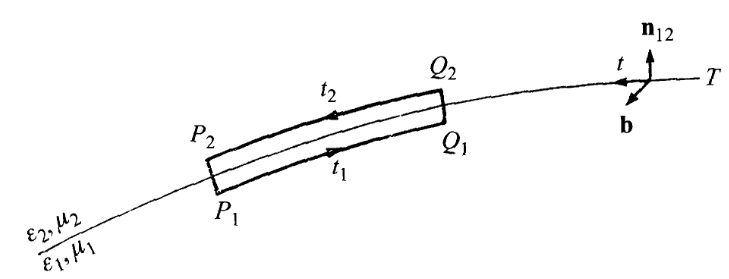
\includegraphics[scale=0.5]{image/fig1-2.png}
		\caption{Derivation of boundary conditions for the tangential components of \textbf{E} and \textbf{H}.}
		\label{fig:1-2}
	\end{figure}	
	\begin{equation}
		\mathbf{H^{(1)}\cdot t_1}\delta s1+\mathbf{H^{(2)}\cdot t_2}\delta s2+\text{contribution from ends}=\frac{1}{c}\mathbf{\dot{D}\cdot b}\delta s\delta h+\frac{4\pi}{c}\mathbf{\hat{j}\cdot b}\delta s.
		\label{1-24}
	\end{equation}
	On proceeding to the limit $\delta h\rightarrow0$ as before, we obtain
	\begin{equation}
		\mathbf{n_{12}}\times(\mathbf{H^{(2)}}-\mathbf{H^{(1)}})=\frac{4\pi}{c}\mathbf{\hat{j}}.
		\label{1-25}
	\end{equation}
	From \eqref{1-25} is follows that \textit{in the presence of a surface current of density} \textbf{j}, \textit{the	tangential component (considered as a vector quantity) of the magnetic vector changes	abruptly, its discontinuity being} $(4\pi/c)\mathbf{\hat{j}}\times\mathbf{n_{12}}$.\par 	Apart from discontinuities due to the abrupt changes in the physical properties of	the medium, the field vectors may also be discontinuous because of the presence of asource which begins to radiate at a particular instant of time $t=t_0$. The disturbance then spreads into the surrounding space, and at any later instant $t_1>t_0$ will have filled a well-defined region. Across the (moving) boundary of this region, the field vectors	will change abruptly from finite values on the boundary to the value zero outside it.\par 
	The various cases of discontinuity may be covered by rewriting Maxwell's equations	in an integral form.\footnote{See, for example, A. Sommerfeld, \textit{Electrodynamics} (New York, Academic Press, 1952), p.11; or J. A.	Stratton, \textit{Electromagnetic Theory} (New York, McGraw-Hill, 1941), p. 6.} The general discontinuity conditions may also be written in the form of simple difference equations; a derivation of these equations is given in	Appendix VI.
	
	\subsection{The energy law of the electromagnetic}
	Electromagnetic theory interprets the light intensity as the energy flux of the field. It is
	therefore necessary to recall the energy law of Maxwell's theory.\par 
	From \eqref{1-1} and \eqref{1-2} it follows that
	\begin{equation}
		\mathbf{E}\cdot curl\ \mathbf{H}-\mathbf{H}\cdot curl\ \mathbf{E}=\frac{4\pi}{c}\mathbf{j\cdot E}+\frac{1}{c}\mathbf{E\cdot\dot{D}}+\frac{1}{c}\mathbf{H\cdot\dot{B}}.
		\label{1-26}
	\end{equation}
	Also, by a well-known vector identity, the term on the left may be expressed as the	divergence of the vector product of \textbf{H} and \textbf{E}:
	\begin{equation}
		\mathbf{E}\cdot curl\ \mathbf{H}-\mathbf{H}\cdot curl\ \mathbf{E}=-div(\mathbf{E}\times\mathbf{H}).
		\label{1-27}
	\end{equation}
	From \eqref{1-26} and \eqref{1-27} we have that
	\begin{equation}
		\frac{1}{c}(\mathbf{E\cdot\dot{D}}+\mathbf{H\cdot\dot{B}})+\frac{4\pi}{c}\mathbf{j\cdot E}+div(\mathbf{E}\times\mathbf{H})=0.
		\label{1-28}
	\end{equation}
	When we multiply this equation by $c/4\pi$, integrate throughout an arbitrary volume and
	apply Gauss's theorem, this gives
	\begin{equation}
		\frac{1}{4\pi}\int(\mathbf{E\cdot\dot{D}}+\mathbf{H\cdot\dot{B}})dV+\int\mathbf{j\cdot E}dV+\frac{c}{4\pi}\int(\mathbf{E}\times\mathbf{H})\cdot\mathbf{n}dS=0,
		\label{1-29}
	\end{equation}
	where the last integral is taken over the boundary of the volume, \textbf{n} being the unit
	outward normal.\par 
	The relation \eqref{1-29} is a direct consequence of Maxwell's equations and is therefore valid whether or not the material equations (\ref{1-9}-\ref{1-11}) hold. It represents, as will be	seen, the energy law of an electromagnetic field. We shall discuss it here only for the	case where the material equations (\ref{1-9}-\ref{1-11}) are satisfied. Generalizations to anisotropic	media, where the material equations are of a more complicated form, will be considered later (Chapter XV).\par 
	We have, on using the material equations,
	\begin{equation}
		\left. \begin{aligned}
		\frac{1}{4\pi}(\mathbf{E\cdot\dot{D}})&=\frac{1}{4\pi}\mathbf{E}\cdot\frac{\partial}{\partial t}(\varepsilon\mathbf{E})&=\frac{1}{8\pi}\frac{\partial}{\partial t}(\varepsilon\mathbf{E}^{2})&=\frac{1}{8\pi}\frac{\partial}{\partial t}(\mathbf{E\cdot D}),\\
		\frac{1}{4\pi}(\mathbf{H\cdot\dot{B}})&=\frac{1}{4\pi}\mathbf{H}\cdot\frac{\partial}{\partial t}(\varepsilon\mathbf{H})&=\frac{1}{8\pi}\frac{\partial}{\partial t}(\varepsilon\mathbf{H}^{2})&=\frac{1}{8\pi}\frac{\partial}{\partial t}(\mathbf{H\cdot B}).	
		\end{aligned}\right\}
		\label{1-30}
	\end{equation}
	Setting
	\begin{equation}
		w_e=\frac{1}{8\pi}\mathbf{E\cdot D},\qquad w_m=\frac{1}{8\pi}\mathbf{H\cdot B},
		\label{1-31}
	\end{equation}
	and
	\begin{equation}
		W=\int(w_e+w_m)dV,
		\label{1-32}
	\end{equation}
	\eqref{1-29} becomes,
	\begin{equation}
		\frac{dW}{dt}+\int\mathbf{j\cdot E}dV+\frac{c}{4\pi}\int(\mathbf{E}\times\mathbf{H})\cdot\mathbf{n}dS=0.
		\label{1-33}
	\end{equation}
	We shall show that W represents the total energy contained within the volume, so that
	$w_e$ may be identified with the \textit{electric energy density} and $w_m$ with the \textit{magnetic energy	density} of the field.\footnote{In the general case the densities are defined by the expressions
	\begin{equation*}
		w_e=\frac{1}{4\pi}\int\mathbf{E\cdot}d\mathbf{D},\qquad w_m=\frac{1}{4\pi}\int\mathbf{H\cdot}d\mathbf{B}.
\end{equation*}
	When the relationship between \textbf{E} and \textbf{D} and between \textbf{H} and \textbf{B} is linear, as here assumed, these expressions reduce to \eqref{1-31}.}
	To justify the interpretation of \textit{W} as the total energy we have to show that, for a	closed system (i.e. one in which the field on the boundary surface may be neglected), the change in \textit{W} as defined above is due to the work done by the field on the material charged bodies which are embedded in it. It suffices to do this for slow motion of the material bodies, which themselves may be assumed to be so small that they can be regarded as point charges $e_k(k=1, 2, \dots)$. Let the velocity of the charge $e_k$ be $\mathbf{v}_k(|\mathbf{v}_k|\ll c)$.\par 
	The force exerted by a field $(\mathbf{E}, \mathbf{B})$ on a charge e moving with velocity \textbf{v} is given by the so-called Lorentz law,
	\begin{equation}
		\mathbf{F}=e\left(\mathbf{E}+\frac{1}{c}\mathbf{v}\times\mathbf{B}\right),
		\label{1-34}
	\end{equation}
	which is based on experience. It follows that if all the charges $e_k$ are displaced by $\delta x_k
	(k =1, 2, \dots)$ in time öt, the total work done is
	\begin{equation*}
		\begin{aligned}
		\delta A=&\sum_{k}\mathbf{F_k}\cdot\delta\mathbf{x_k}=\sum_{k}e_k\left(\mathbf{E_k}+\frac{1}{c}\mathbf{v_k}\times\mathbf{B}\right)\cdot\delta\mathbf{x_k}\\
		=&\sum_{k}e_k\mathbf{E_k}\cdot\delta\mathbf{x_k}=\sum_{k}e^k\mathbf{E_k}\cdot\mathbf{v_k}\delta t,
		\end{aligned}
	\end{equation*}
	since $\delta\mathbf{x_k} =\mathbf{v_k}\delta t$. If the number of charged particles is large, we can consider the distribution to be continuous. We introduce the charge density p (i.e. total charge per	unit volume) and the last equation becomes
	\begin{equation}
		\delta A=\delta t\int\rho\mathbf{v\cdot E}dV,
		\label{1-35}
	\end{equation}
	the integration being carried throughout an arbitrary volume. Now the velocity v does not appear explicitly in Maxwell's equations, but it may be introduced by using an	experimental result found by Röntgen\footnote{W. C. Röntgen, Ann. d. Physik, 35 A888), 264; 40 A890), 93.}, according to which a \textit{convection current} (i.e. a	set of moving charges) has the same electromagnetic effect as a \textit{conduction current} in a wire. Hence the current density \textbf{j} appearing in Maxwell's equations can be split into two parts
	\begin{equation}
		\mathbf{j}=\mathbf{j_c}+\mathbf{j_\upsilon},
		\label{1-36}
	\end{equation}
	where
	$$\mathbf{j_c}=\sigma\mathbf{E}$$
	is the conduction current density, and
	$$\mathbf{j_\upsilon}=\rho\mathbf{v}$$
	represents the convection current density. \eqref{1-35} may therefore be written as
	\begin{equation}
		\delta A=\delta t\int\mathbf{j_\upsilon\cdot E}dV.
		\label{1-37}
	\end{equation}
	Let us now define a vector \textbf{S} and a scalar Q by the relations
	\begin{equation}
		\mathbf{S}=\frac{c}{4\pi}(\mathbf{E}\times\mathbf{H}),
		\label{1-38}
	\end{equation}
	\begin{equation}
		Q=\int\mathbf{j_c\cdot E}dV=\int\sigma\mathbf{E}^2dV.
		\label{1-39}
	\end{equation}
	then by \eqref{1-35} and \eqref{1-36}
	\begin{equation}
	\begin{aligned}
	\int\mathbf{j\cdot E}dV=&Q+\int\mathbf{j_\upsilon\cdot E}dV\\
	=&Q+\frac{\delta A}{\delta t}
	\end{aligned}
	\label{1-40}	
	\end{equation}
	where the second function is not, of course, a total derivative of a space-time function.
	Eq. \eqref{1-33} now takes the form
	\begin{equation}
		\frac{dW}{dt}=-\frac{\delta A}{\delta t}-Q-\int\mathbf{S\cdot n}dS.
		\label{1-41}
	\end{equation}
	For a nonconductor $(\sigma=0)$ we have that $Q=0$. Assume also that the boundary surface is so far away that we can neglect the field on it, due to the electromagnetic processes inside; then $\int\mathbf{S\cdot n}dS=0$, and integration of \eqref{1-41} gives
	\begin{equation}
		W+A=constant.
		\label{1-42}
	\end{equation}
	Hence, for an isolated system, the increase of \textit{W} per unit time is due to the work done on the system during this time. This result justifies our definition of electromagnetic energy by means of \eqref{1-32}.\par 
	The term \textit{Q} represents the resistive dissipation of energy (called \textit{Joule s heat}) in a conductor $(\sigma\neq 0)$. According to \eqref{1-41} there is a further decrease in energy if the field extends to the boundary surface. The surface integral must therefore represent the flow	of energy across this boundary surface. The vector \textbf{S} is known as the \textit{Poynting vector} and represents the amount of energy which crosses per second a unit area normal to the directions of \textbf{E} and \textbf{H}.\par 
	It should be noted that the interpretation of \textbf{S} as energy flow (more precisely as the density of the flow) is an abstraction which introduces a certain degree of arbitrariness.	For the quantity which is physically significant is, according to \eqref{1-41}, not \textbf{S} itself, but the integral of $\mathbf{S\cdot n}$ taken over a closed surface. Clearly, from the value of the integral, no unambiguous conclusion can be drawn about the detailed distribution of \textbf{S}, and alternative definitions of the energy flux density are therefore possible. One can always add to \textbf{S} the curl of an arbitrary vector, since such a term will not contribute to the surface integral as can be seen from Gauss' theorem and the identity $div\ curl\equiv0$.\footnote{According to modern theories of fields the arbitrariness is even greater, allowing for alternative expressions
	for both the energy density and the energy flux, but consistent with the change of the Lagrangian density	of the field by the addition of a four-divergence. For a discussion of this subject see, for example, G.	Wentzel, Quantum Theory of Fields (New York, Interscience Publishers, 1949), especially \S2 or J. D.	Jackson, Classical Electrodynamics (New York, J. Wiley and Sons, 2nd ed. 1975), Sec. 12.10, especially p.602.}	However, when the definition has been applied cautiously, in particular for averages over small but finite regions of space or time, no contradictions with experiments have been found. We shall therefore accept the above definition in terms of the Poynting	vector of the density of the energy flow.\par 
	Finally we note that in a nonconducting medium $(\sigma=0)$ where no mechanical work is done $(A =	0)$, the energy law may be written in the form of a hydrodynamical continuity equation for noncompressible fluids:
	\begin{equation}
		\frac{\partial w}{\partial t}+div\ \mathbf{S}=0,\qquad (w=w_e+w_m).
		\label{1-43}
	\end{equation}
	A description of propagation of light in terms of a hydrodynamical model is often helpful, particularly in the domain of geometrical optics and in connection with scalar diffraction fields, as it gives a picture of the energy transport in a simple and graphic manner. In optics, the (averaged) Poynting vector is the chief quantity of interest. The magnitude of the Poynting vector is a measure of the light intensity, and its direction represents the direction of propagation of the light.
	
	
	\section{The wave equation and the velocity of light}
	Maxwell's equations relate the field vectors by means of simultaneous differential equations. On elimination we obtain differential equations which each of the vectors must separately satisfy. We shall confine our attention to that part of the field which contains no charges or currents, i.e. where $\bf{j}=0$ and $\rho=0$.\par 
	We substitute for B from the material equation \S§1.1 \eqref{1-11} into the second Maxwell equation \S1.1 \eqref{1-12}, divide both sides by ju and apply the operator curl. This gives
	\setcounter{equation}{0}
	\begin{equation}
		curl\ \left(\frac{1}{\mu}curl\ \mathbf{E}\right)+\frac{1}{c}curl\ \bf{\dot{H}}=0.
		\label{2-1}
	\end{equation}
\end{document}